% \documentclass[12pt]{article}
% \begin{document}
\documentclass[aspectratio=169, 11pt]{beamer}
\usepackage{tikz}
\usetheme{Copenhagen}
\usecolortheme{beaver}

\usepackage{booktabs}
\usepackage{graphicx}
\graphicspath{ {img/} }

\begin{document}
\title{Project 2}   
\author{
B03902003 Chia-sheng Chen\\
B03902036 Yen-ting Liu\\
B03902104 Yi-ying Chao} 
\date{\today} 
\frame{\titlepage}

\frame{\frametitle{Table of contents}\tableofcontents} 

\section{L1 Cache}
\subsection{L1 Cache Structure}
\begin{frame}
  \frametitle{System Block Diagram}
  \includegraphics[width=\textwidth]{systemBlockDiagram}\\
  \footnotesize{\# From TA}
\end{frame}

\begin{frame}
  \frametitle{L1 Cache Structure}
  \includegraphics{cacheStructure}
\end{frame}


\subsection{Read and Write of Cache}
\begin{frame}
  \frametitle{Example of Read and Write Structure}
  \includegraphics[height=0.85\textheight]{readWrite}
\end{frame}

\begin{frame}
  \frametitle{Difference}
  \begin{itemize}
  \item 8 Mux instead of 4 Mux when write (8 words in a cache line)
  \item 31:10 tag bit, 9:5 index bit, 4:0 offset bit (spec) 
  \end{itemize}
\end{frame}

\begin{frame}
  \frametitle{Deciding the Source of Data}
  \begin{table}[]
  \centering
  \caption{Deciding the Source of Data}
  \label{my-label}
  \begin{tabular}{@{}lll@{}}
  \toprule
             & Load Word (Read)     & Store Word (Write)                 \\ \midrule
  Cache  Hit & Every word from SRAM & One word from CPU, other from SRAM \\
  Cache Miss & Every word from DRAM & One word from CPU, other from DRAM \\ \bottomrule
  \end{tabular}
  \end{table}
\end{frame}

\tiny
\subsection{Inside Cache Controller}
\begin{frame}
  \frametitle{Finite State Machine}

\begin{center}
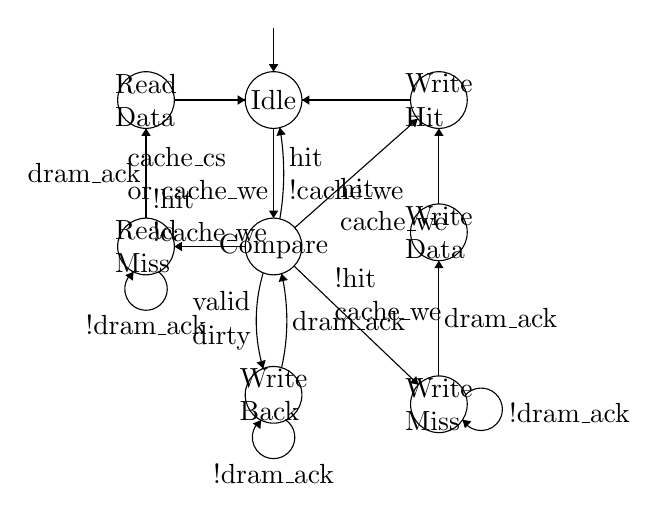
\begin{tikzpicture}[scale=0.12]
\tikzstyle{every node}+=[inner sep=0pt]
\draw [black] (33.1,-9.2) circle (3);
\draw (33.1,-9.2) node {Idle};
\draw [black] (33.1,-24.7) circle (3);
\draw (33.1,-24.7) node {Compare};
\draw [black] (19.6,-24.7) circle (3);
\draw (19.6,-24.7) node [align=left] {Read\\Miss};
\draw [black] (19.6,-9.2) circle (3);
\draw (19.6,-9.2) node [align=left] {Read\\Data};
\draw [black] (33.1,-40.4) circle (3);
\draw (33.1,-40.4) node [align=left] {Write\\Back};
\draw [black] (50.6,-41.4) circle (3);
\draw (50.6,-41.4) node [align=left] {Write\\Miss};
\draw [black] (50.6,-9.2) circle (3);
\draw (50.6,-9.2) node [align=left] {Write\\Hit};
\draw [black] (50.6,-23.2) circle (3);
\draw (50.6,-23.2) node [align=left] {Write\\Data};
\draw [black] (33.1,-1.6) -- (33.1,-6.2);
\fill [black] (33.1,-6.2) -- (33.6,-5.4) -- (32.6,-5.4);
\draw [black] (33.764,-12.124) arc (9.77504:-9.77504:28.424);
\fill [black] (33.76,-12.12) -- (33.41,-13) -- (34.39,-12.83);
\draw (34.68,-16.95) node [right, align=left] {hit\\!cache\_we};
\draw [black] (33.1,-12.2) -- (33.1,-21.7);
\fill [black] (33.1,-21.7) -- (33.6,-20.9) -- (32.6,-20.9);
\draw (32.6,-16.95) node [left, align=left] {cache\_cs\\or cache\_we};
\draw [black] (30.1,-24.7) -- (22.6,-24.7);
\fill [black] (22.6,-24.7) -- (23.4,-25.2) -- (23.4,-24.2);
\draw (26.35,-24.2) node [above, align=left] {!hit\\!cache\_we};
\draw [black] (19.6,-21.7) -- (19.6,-12.2);
\fill [black] (19.6,-12.2) -- (19.1,-13) -- (20.1,-13);
\draw (19.1,-16.95) node [left] {dram\_ack};
\draw [black] (22.6,-9.2) -- (30.1,-9.2);
\fill [black] (30.1,-9.2) -- (29.3,-8.7) -- (29.3,-9.7);
\draw [black] (32.005,-37.611) arc (-163.41994:-196.58006:17.735);
\fill [black] (32.01,-37.61) -- (32.26,-36.7) -- (31.3,-36.99);
\draw (30.77,-32.55) node [left, align=left] {valid\\dirty};
\draw [black] (35.27,-26.77) -- (48.43,-39.33);
\fill [black] (48.43,-39.33) -- (48.2,-38.41) -- (47.51,-39.14);
\draw (45.22,-32.57) node [above, align=left] {!hit\\cache\_we};
\draw [black] (50.6,-38.4) -- (50.6,-26.2);
\fill [black] (50.6,-26.2) -- (50.1,-27) -- (51.1,-27);
\draw (51.1,-32.3) node [right] {dram\_ack};
\draw [black] (50.6,-20.2) -- (50.6,-12.2);
\fill [black] (50.6,-12.2) -- (50.1,-13) -- (51.1,-13);
\draw [black] (35.35,-22.71) -- (48.35,-11.19);
\fill [black] (48.35,-11.19) -- (47.42,-11.35) -- (48.09,-12.09);
\draw (45.81,-17.44) node [below, align=left] {hit\\cache\_we};
\draw [black] (47.6,-9.2) -- (36.1,-9.2);
\fill [black] (36.1,-9.2) -- (36.9,-9.7) -- (36.9,-8.7);
\draw [black] (53.418,-40.405) arc (137.17202:-150.82798:2.25);
\draw (57.97,-42.33) node [right] {!dram\_ack};
\fill [black] (53.1,-43.03) -- (53.35,-43.94) -- (54.03,-43.21);
\draw [black] (34.423,-43.08) arc (54:-234:2.25);
\draw (33.1,-47.65) node [below] {!dram\_ack};
\fill [black] (31.78,-43.08) -- (30.9,-43.43) -- (31.71,-44.02);
\draw [black] (20.923,-27.38) arc (54:-234:2.25);
\draw (19.6,-31.95) node [below] {!dram\_ack};
\fill [black] (18.28,-27.38) -- (17.4,-27.73) -- (18.21,-28.32);
\draw [black] (33.952,-27.574) arc (12.71147:-12.71147:22.613);
\fill [black] (33.95,-27.57) -- (33.64,-28.46) -- (34.62,-28.24);
\draw (35.01,-32.55) node [right] {dram\_ack};
\end{tikzpicture}
\end{center}
\end{frame}

\section{DRAM}
\frame{
  \frametitle{FSM}

\begin{center}
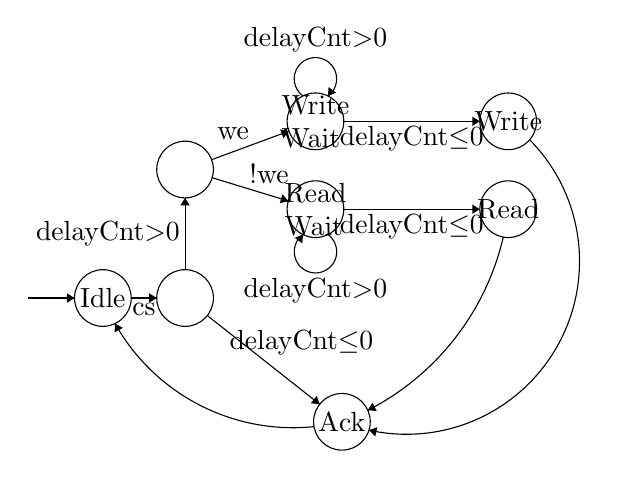
\begin{tikzpicture}[scale=0.12]
\tikzstyle{every node}+=[inner sep=0pt]
\draw [black] (13,-32.5) circle (3);
\draw (13,-32.5) node {Idle};
\draw [black] (35.5,-23.1) circle (3);
\draw (35.5,-23.1) node [align=left] {Read\\Wait};
\draw [black] (35.5,-13.8) circle (3);
\draw (35.5,-13.8) node [align=left] {Write\\Wait};
\draw [black] (55.9,-13.8) circle (3);
\draw (55.9,-13.8) node {Write};
\draw [black] (38.3,-45.6) circle (3);
\draw (38.3,-45.6) node {Ack};
\draw [black] (55.9,-23.1) circle (3);
\draw (55.9,-23.1) node {Read};
\draw [black] (21.7,-32.5) circle (3);
\draw [black] (21.7,-18.9) circle (3);
\draw [black] (5.1,-32.5) -- (10,-32.5);
\fill [black] (10,-32.5) -- (9.2,-32) -- (9.2,-33);
\draw [black] (16,-32.5) -- (18.7,-32.5);
\fill [black] (18.7,-32.5) -- (17.9,-32) -- (17.9,-33);
\draw (17.35,-33) node [below] {cs};
\draw [black] (21.7,-29.5) -- (21.7,-21.9);
\fill [black] (21.7,-21.9) -- (21.2,-22.7) -- (22.2,-22.7);
\draw (21.2,-25.7) node [left] {delayCnt$>$0};
\draw [black] (24.06,-34.36) -- (35.94,-43.74);
\fill [black] (35.94,-43.74) -- (35.63,-42.85) -- (35.01,-43.64);
\draw (34.01,-38.55) node [above] {delayCnt$\leq$0};
\draw [black] (24.51,-17.86) -- (32.69,-14.84);
\fill [black] (32.69,-14.84) -- (31.76,-14.65) -- (32.11,-15.59);
\draw (26.78,-15.8) node [above] {we};
\draw [black] (24.57,-19.77) -- (32.63,-22.23);
\fill [black] (32.63,-22.23) -- (32.01,-21.52) -- (31.72,-22.47);
\draw (30.58,-20.39) node [above] {!we};
\draw [black] (36.823,-25.78) arc (54:-234:2.25);
\draw (35.5,-30.35) node [below] {delayCnt$>$0};
\fill [black] (34.18,-25.78) -- (33.3,-26.13) -- (34.11,-26.72);
\draw [black] (34.177,-11.12) arc (234:-54:2.25);
\draw (35.5,-6.55) node [above] {delayCnt$>$0};
\fill [black] (36.82,-11.12) -- (37.7,-10.77) -- (36.89,-10.18);
\draw [black] (38.5,-23.1) -- (52.9,-23.1);
\fill [black] (52.9,-23.1) -- (52.1,-22.6) -- (52.1,-23.6);
\draw (45.7,-23.6) node [below] {delayCnt$\leq$0};
\draw [black] (38.5,-13.8) -- (52.9,-13.8);
\fill [black] (52.9,-13.8) -- (52.1,-13.3) -- (52.1,-14.3);
\draw (45.7,-14.3) node [below] {delayCnt$\leq$0};
\draw [black] (55.379,-26.053) arc (-13.1233:-62.94332:27.626);
\fill [black] (41.04,-44.38) -- (41.98,-44.46) -- (41.53,-43.57);
\draw [black] (58.172,-15.754) arc (44.6111:-102.53657:18.311);
\fill [black] (41.16,-46.49) -- (41.83,-47.15) -- (42.05,-46.17);
\draw [black] (35.347,-46.113) arc (-84.11911:-150.62991:21.625);
\fill [black] (14.29,-35.21) -- (14.24,-36.15) -- (15.11,-35.66);
\end{tikzpicture}
\end{center}
}

\end{document}

